% Copyright 2004 by Till Tantau <tantau@users.sourceforge.net>.
%
% In principle, this file can be redistributed and/or modified under
% the terms of the GNU Public License, version 2.
%
% However, this file is supposed to be a template to be modified
% for your own needs. For this reason, if you use this file as a
% template and not specifically distribute it as part of a another
% package/program, I grant the extra permission to freely copy and
% modify this file as you see fit and even to delete this copyright
% notice. 

\documentclass{beamer}
\usepackage{tikz}
\usepackage{booktabs}
\usepackage{tcolorbox}
\usepackage{wrapfig}


\usetikzlibrary{matrix}
\newcommand{\cX}{\mathcal{X}}
\newcommand{\cY}{\mathcal{Y}}
\newcommand{\cO}{\mathcal{O}}
\newcommand{\cC}{\mathcal{C}}
\newcommand{\cD}{\mathcal{D}}
\newcommand{\cW}{\mathcal{W}}
\newcommand{\cG}{\mathcal{G}}

% There are many different themes available for Beamer. A comprehensive
% list with examples is given here:
% http://deic.uab.es/~iblanes/beamer_gallery/index_by_theme.html
% You can uncomment the themes below if you would like to use a different
% one:
%\usetheme{AnnArbor}
%\usetheme{Antibes}
%\usetheme{Bergen}
%\usetheme{Berkeley}
%\usetheme{Berlin}
%\usetheme{Boadilla}
%\usetheme{boxes}
%\usetheme{CambridgeUS}
%\usetheme{Copenhagen}
%\usetheme{Darmstadt}
\usetheme{default}
%\usetheme{Frankfurt}
%\usetheme{Goettingen}
%\usetheme{Hannover}
%\usetheme{Ilmenau}
%\usetheme{JuanLesPins}
%\usetheme{Luebeck}
%\usetheme{Madrid}
%\usetheme{Malmoe}
%\usetheme{Marburg}
%\usetheme{Montpellier}
%\usetheme{PaloAlto}
%\usetheme{Pittsburgh}
%\usetheme{Rochester}
%\usetheme{Singapore}
%\usetheme{Szeged}
%\usetheme{Warsaw}

\title{On the (im)possibility of fairness}
\subtitle{Sorelle A. Friedler, Carlos Scheidegger, Suresh Venkatasubramanian}

% A subtitle is optional and this may be deleted

\author{presented by Sarah Dean}

% - Give the names in the same order as the appear in the paper.
% - Use the \inst{?} command only if the authors have different
%   affiliation.

% \institute[Universities of Somewhere and Elsewhere] % (optional, but mostly needed)
% {
%   \inst{1}%
%   Department of Computer Science\\
%   University of Somewhere
%   \and
%   \inst{2}%
%   Department of Theoretical Philosophy\\
%   University of Elsewhere}
% % - Use the \inst command only if there are several affiliations.
% % - Keep it simple, no one is interested in your street address.

\date{Fairness in ML, September 2017}
% - Either use conference name or its abbreviation.
% - Not really informative to the audience, more for people (including
%   yourself) who are reading the slides online

\subject{Theoretical Computer Science}
% This is only inserted into the PDF information catalog. Can be left
% out. 

% If you have a file called "university-logo-filename.xxx", where xxx
% is a graphic format that can be processed by latex or pdflatex,
% resp., then you can add a logo as follows:

%\pgfdeclareimage[height=0.5cm]{university-logo}{ucbseal.png}
%\logo{\pgfuseimage{university-logo}}

% Delete this, if you do not want the table of contents to pop up at
% the beginning of each subsection:
% \AtBeginSubsection[]
% {
%   \begin{frame}<beamer>{Outline}
%     \tableofcontents[currentsection,currentsubsection]
%   \end{frame}
% }

% Let's get started
\begin{document}

\begin{frame}
  \titlepage
\end{frame}

% \begin{frame}{Outline}
%   \tableofcontents
%   % You might wish to add the option [pausesections]
% \end{frame}

% Section and subsections will appear in the presentation overview
% and table of contents.
\section{First Main Section}

\subsection{First Subsection}

\begin{frame}{``Similar people should be treated similarly"}{~~~~~~but similar in what sense?}

On Monday, we considered the fairness constraint
\[D(f(x),f(x')) \leq d(x,x')\]
which amounts to a Lipschitz condition on the decision map $f:\cX\to \cD$
\pause

  \begin{itemize}
  \item {
    Sensitivity to definition of $d$
  }
  \item{
    What is the space of individuals $\cal{X}$? The feature space?
  }
  \end{itemize}
\end{frame}

% You can reveal the parts of a slide one at a time
% with the \pause command:
\begin{frame}{Three spaces of the decision pipeline}
We distinguish between the {\it construct space} $\cC$, the {\it observed space} $\cO$, and the {\it decision space} $\cD$ .

\begin{table}[h!]
  \centering
  \label{tab:table1}
  \begin{tabular}{ccc}
    \toprule
    Decision space & Construct space & Observed space\\
    \midrule
    College performance & intelligence & IQ\\
    College performance & HS success & GPA\\
    Recidivism & ``criminality'' & family history of crime\\
    Recidivism & risk-averseness & age\\
    Employee productivity & knowedge of job & years experience\\
    \bottomrule
  \end{tabular}
\end{table}


\pause
  \begin{itemize}
  \item{
    Imperfections in choice of construct vs. observed space?
  }
  \item<3->{
    Should we distinguish between the decision space (label space) and the outcome space?
  }
  \end{itemize}
\end{frame}

\begin{frame}{Decision pipeline as maps between spaces}


\begin{columns}[T]
 \column{0.99\textwidth}
We consider transformations between spaces,
  \begin{itemize}
  \item{
    observation processes $g:\cC\to\cO$
  }
  \item{
    desired ``ideal map'' $f:\cC\to\cD$
  }  
  \item{
    designed or learned map $\hat f:\cO\to\cD$
  }
  \end{itemize}




 \column{0.01\textwidth}
 \hspace*{-4cm}
 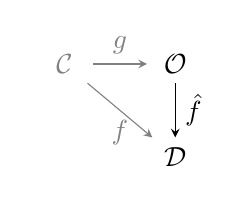
\begin{tikzpicture}[ampersand replacement=\&]
  \matrix(m)[matrix of math nodes,row sep=2em,column sep=2em,minimum width=2em]
  { {\color{gray}\cC} \& \cO \\
     \& \cD\\};
  \path[-stealth, gray]
    (m-1-1) edge node [above] {$g$} (m-1-2) edge node [below] {$f$} (m-2-2);
  \path[-stealth]
    (m-1-2) edge node [right] {$\hat f$} (m-2-2);
\end{tikzpicture}
\end{columns}
\pause %to what extent do mappings {\it define} the spaces?

\vspace{1cm}
To make up for lack of knowledge about $\cC$, $g$, and $f$, we will have to make assumptions based on our ``world view''. 
\uncover<3->{\noindent\rule{\textwidth}{1pt}

The {\bf distortion} $\rho_h$ of map $h:\cX\to\cY$ is
\[\sup_{x,x'\in\cX} |d_\cX(x,x')-d_\cY(h(x),h(x'))|\]
and $\rho(\cX,\cY)=\min_{h}\rho_h$

}
%to what extent do maps DETERMINE the spaces? Are spaces empirically made up of individuals, or an entire space (like R2?)
  
%    Fifth item. \uncover<6->{Extra text in the fifth item.}

\end{frame}


\begin{frame}{Individual fairness and what-you-see-is-what-you-get}


A map $f:\cC\to\cD$ is ($\epsilon, \epsilon'$)-{\bf fair} if for all $x,x'\in\cC$
\[d_\cC(x,x')\leq \epsilon \implies d_\cD(f(x),f(x'))\leq\epsilon'\]

\pause \vspace{0.5cm}
\begin{tcolorbox}
{\bf Axiom} (WYSIWYG) The distortion between $\cC$ and $\cO$ is at most $\delta$
\end{tcolorbox}
\vspace{0.5cm}
\uncover<3->{An {\bf individual fairness mechanism} (IFM$_\epsilon$) is a nontrivial mapping  $\hat{f}:\cO\to\cD$ with $\rho_{\hat {f}} \leq \epsilon$.
}

%    Fifth item. \uncover<6->{Extra text in the fifth item.}

\end{frame}
\begin{frame}{Fairness is possible!!!}

\begin{tcolorbox}
\begin{theorem}
Under WYSIWYG, an IFM$_{\delta'}$  guarantees ($\epsilon, \delta+\delta'$)-fairness.
\end{theorem}
\end{tcolorbox}
\begin{center}
 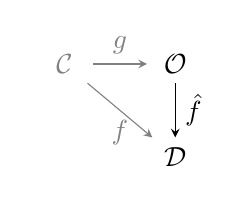
\begin{tikzpicture}[ampersand replacement=\&]
  \matrix(m)[matrix of math nodes,row sep=2em,column sep=2em,minimum width=2em]
  { {\color{gray}\cC} \& \cO \\
     \& \cD\\};
  \path[-stealth, gray]
    (m-1-1) edge node [above] {{$g$}} (m-1-2) edge node [below] {$f$} (m-2-2);
  \path[-stealth]
    (m-1-2) edge node [right] {$\hat f$} (m-2-2);
\end{tikzpicture}
\end{center}

%    Fifth item. \uncover<6->{Extra text in the fifth item.}

\end{frame}

\begin{frame}{Fairness is possible!!!}

\begin{tcolorbox}
\begin{theorem}
Under {\color{red}{WYSIWYG}}, an {\color{blue} IFM$_{\delta'}$}  guarantees ($\epsilon, \delta+\delta'$)-{\color{green}fairness}.
\end{theorem}
\end{tcolorbox}
\begin{center}
 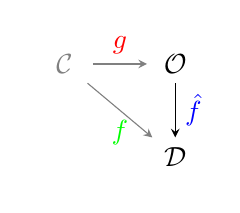
\begin{tikzpicture}[ampersand replacement=\&]
  \matrix(m)[matrix of math nodes,row sep=2em,column sep=2em,minimum width=2em]
  { {\color{gray}\cC} \& \cO \\
     \& \cD\\};
  \path[-stealth, gray]
    (m-1-1) edge node [above] {\color{red}{$g$}} (m-1-2) edge node [below] {\color{green} $f$} (m-2-2);
  \path[-stealth]
    (m-1-2) edge node [right] {\color{blue}$\hat f$} (m-2-2);
\end{tikzpicture}
\end{center}

%    Fifth item. \uncover<6->{Extra text in the fifth item.}

\end{frame}

\begin{frame}{Fairness is impossible :(}

\begin{tcolorbox}
\begin{theorem}
Under WYSIWYG($\epsilon$), any nontrivial map $\hat f:\cO\to\cD$ is not $(\delta-\epsilon, \delta')$-fair for any $\delta,\delta'<1$ if $\cD$ is discrete
\end{theorem}

\end{tcolorbox}
\pause
\begin{center}
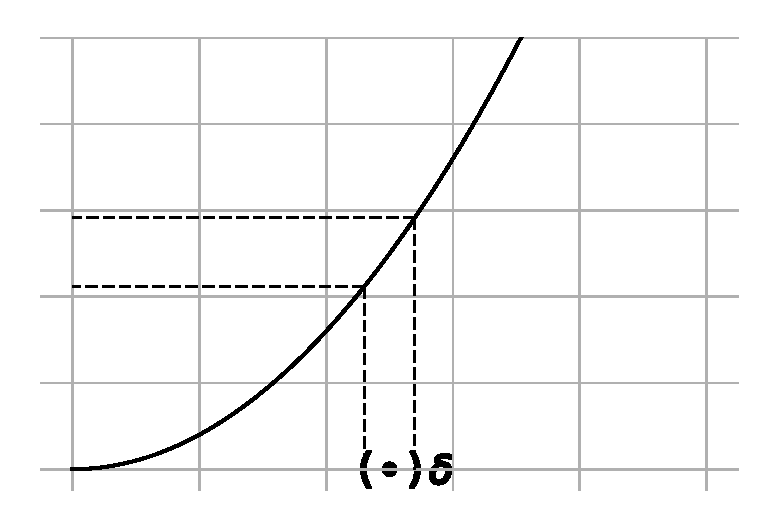
\includegraphics[width=0.4\textwidth]{conts.eps} 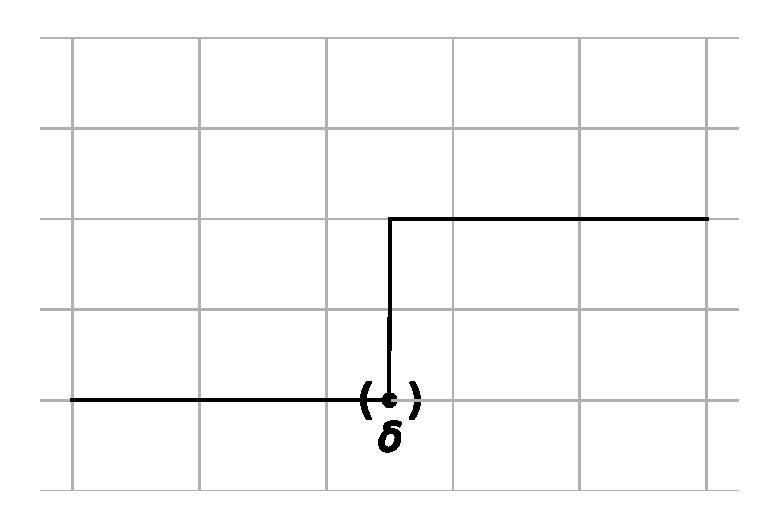
\includegraphics[width=0.4\textwidth]{disconts.eps} 
\end{center}

  \begin{itemize}
  \item{
    What about randomization?
  }
  \end{itemize}
  
\end{frame}

%    Fifth item. \uncover<6->{Extra text in the fifth item.}



\begin{frame}{Beyond individuals: structural bias}
\begin{columns}[T]
 \column{0.8\textwidth}
How might bias against certain groups manifest itself in this framework?
\begin{itemize}
\item Individuals belong to groups, partitioning the space $\cC = X_1\cup...\cup X_k$, $\cO = Y_1\cup...\cup Y_k$
\end{itemize}
 \column{0.2\textwidth}
 \hspace*{-0.5cm}
 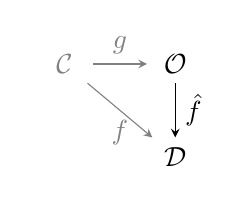
\begin{tikzpicture}[ampersand replacement=\&]
  \matrix(m)[matrix of math nodes,row sep=2em,column sep=2em,minimum width=2em]
  { {\color{gray}\cC} \& \cO \\
     \& \cD\\};
  \path[-stealth, gray]
    (m-1-1) edge node [above] {$g$} (m-1-2) edge node [below] {$f$} (m-2-2);
  \path[-stealth]
    (m-1-2) edge node [right] {$\hat f$} (m-2-2);
\end{tikzpicture}
\end{columns}
\pause \noindent\rule{\textwidth}{1pt}
Measure distance between subsets $X,X'$ in the same space $\cX$ with {\bf Wasserstein distance}
\[\cW_d(X,X') = \min_{\nu \in \mathcal{U}(X,X')} \int d_\cX (x,x')\nu(x,x') \]

\uncover<3->{\noindent\rule{\textwidth}{1pt}
Measure distance between subsets $X,Y$ in the different spaces with {\bf Gromov-Wasserstein distance}
\[\cG(X,Y) = \frac{1}{2}\inf_{\mu } \int |d_\cX (x,x')-d_\cY (y,y')|d\mu_X\times d\mu_Xd\mu_Y\times d\mu_Y \]
}

\end{frame}

\begin{frame}{Structual bias and discrimination}
The {\bf between-groups} and {\bf within-group distances} of $\cX = \bigcup_{i=1}^k X_i$ and $\cY=\bigcup_{i=1}^k Y_i$ are respectively 
\[\rho_b = \frac{1}{\binom{k}{2} }\cG(\cX,\cY),~~ \rho_w = \frac{1}{k}\sum_{i=1}^k \cG(X_i,Y_i) \:,\]
and the {\bf group skew} is
\[\sigma(\cX,\cY) = \frac{\rho_b(\cX,\cY)}{\rho_w(\cX,\cY)}\]
\pause
\noindent\rule{\textwidth}{1pt}

We have \begin{itemize}
\item $t$-{\bf structural bias}: $\sigma(\cC,\cO)>t$
\item $t$-{\bf direct discrimination}: $\sigma(\cO,\cD)>t$
\item a $t$-{\bf nondiscriminatory} mapping $f:\cC\to\cD$ if $\sigma(\cC,\cD)\leq t$
\end{itemize}

\end{frame}

\begin{frame}{Structual bias and discrimination}
How does this notion of structural bias compare with an intuitive one?
\vspace{1cm}


What does direct discrimination look like? Can affirmative action be direct discrimination?
\end{frame}

\begin{frame}{We're all equal}

\begin{columns}[T]

 \column{0.8\textwidth}
If structural bias is suspected, WYSIWYG doesn't hold. How can we get around our lack of knowledge about the construct space?

 \column{0.2\textwidth}
 \hspace*{-0.5cm}
 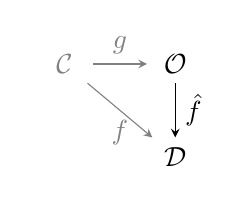
\begin{tikzpicture}[ampersand replacement=\&]
  \matrix(m)[matrix of math nodes,row sep=2em,column sep=2em,minimum width=2em]
  { {\color{gray}\cC} \& \cO \\
     \& \cD\\};
  \path[-stealth, gray]
    (m-1-1) edge node [above] {$g$} (m-1-2) edge node [below] {$f$} (m-2-2);
  \path[-stealth]
    (m-1-2) edge node [right] {$\hat f$} (m-2-2);
\end{tikzpicture}
\end{columns}

\pause
\begin{tcolorbox}
{\bf Axiom} (WAE) For $\cC = X_1\cup...\cup X_k$, 
\[\cW_{d_\cC}(X_i,X_j) < \epsilon~ \text{for all}~ 1\leq i,j\leq k \]
\end{tcolorbox}

\uncover<3->{A {\bf group fairness mechanism} (GFM$_\epsilon$) $f:\cO\to\cD$ with $\cO = Y_1\cup...\cup Y_k$ satisfies $\cW_{d_\cO}( f(Y_i),f(Y_j))\leq \epsilon$ }

\end{frame}

\begin{frame}{Nondiscrimination is possible!}
\begin{tcolorbox}
\begin{theorem}
Under WAE, a GFM$_{\epsilon'}$ guarantees $\frac{\max{(\epsilon,\epsilon')}}{\delta} $-nondiscrimination
\end{theorem}
\end{tcolorbox}
\begin{center}
 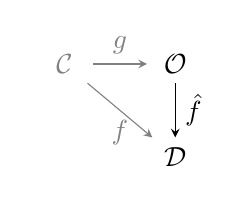
\begin{tikzpicture}[ampersand replacement=\&]
  \matrix(m)[matrix of math nodes,row sep=2em,column sep=2em,minimum width=2em]
  { {\color{gray}\cC} \& \cO \\
     \& \cD\\};
  \path[-stealth, gray]
    (m-1-1) edge node [above] {$g$} (m-1-2) edge node [below] {$f$} (m-2-2);
  \path[-stealth]
    (m-1-2) edge node [right] {$\hat f$} (m-2-2);
\end{tikzpicture}
\end{center}

\end{frame}

\begin{frame}{Nondiscrimination is possible!}
\begin{tcolorbox}
\begin{theorem}
Under {\color{red}WAE}, a {\color{blue}GFM$_{\epsilon'}$} guarantees $\frac{\max{(\epsilon,\epsilon')}}{\delta} $-{\color{green}nondiscrimination}
\end{theorem}
\end{tcolorbox}
\begin{center}
 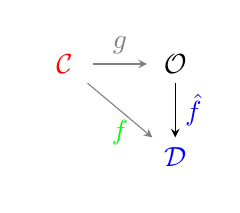
\begin{tikzpicture}[ampersand replacement=\&]
  \matrix(m)[matrix of math nodes,row sep=2em,column sep=2em,minimum width=2em]
  { {\color{red}\cC} \& \cO \\
     \& {\color{blue}\cD}\\};
  \path[-stealth, gray]
    (m-1-1) edge node [above] {$g$} (m-1-2) edge node [below] {\color{green} $f$} (m-2-2);
  \path[-stealth]
    (m-1-2) edge node [right] {\color{blue} $\hat f$} (m-2-2);
\end{tikzpicture}
\end{center}

\pause
Could achieving nondiscrimination in this setting require direct discrimination?

\end{frame}




\begin{frame}{Worldview comparison}{WYSIWYG vs. WAE}

Each axiom induces fairness mechanism (group v. individual) to achieve fairness or nondiscrimination. Are they always incompatible?

\pause 
\vspace{0.5cm}
How can we understand the following as part of this framework?
\begin{itemize}
  \item Observational measures: \begin{itemize}
    \item demographic parity (equalized odds)
    \item accuracy parity 
    \item true positive parity (equal opportunity)
    \item predictive value parity 
  \end{itemize}
  \item Credit scores?
  \item COMPAS: Kristian Lum's approach
\end{itemize}


\end{frame}


\begin{frame}{Beyond conceptual design?}


\begin{columns}[T]

 \column{0.5\textwidth}
 \begin{center}
 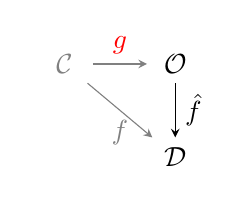
\begin{tikzpicture}[ampersand replacement=\&]
  \matrix(m)[matrix of math nodes,row sep=2em,column sep=2em,minimum width=2em]
  { {\color{gray}\cC} \& \cO \\
     \& \cD\\};
  \path[-stealth, gray]
    (m-1-1) edge node [above] {\color{red} $g$} (m-1-2) edge node [below] {$f$} (m-2-2);
  \path[-stealth]
    (m-1-2) edge node [right] {$\hat f$} (m-2-2);
\end{tikzpicture}

 {\color{red} Assume good observations}

\end{center}
 \column{0.5\textwidth}
 \begin{center}
 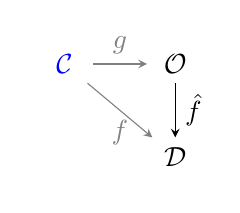
\begin{tikzpicture}[ampersand replacement=\&]
  \matrix(m)[matrix of math nodes,row sep=2em,column sep=2em,minimum width=2em]
  { {\color{blue}\cC} \& \cO \\
     \& \cD\\};
  \path[-stealth, gray]
    (m-1-1) edge node [above] {$g$} (m-1-2) edge node [below] {$f$} (m-2-2);
  \path[-stealth]
    (m-1-2) edge node [right] {$\hat f$} (m-2-2);
\end{tikzpicture}

{\color{blue} Assume inherent equality}
\end{center}
\end{columns}
\vspace{0.5cm}


Framework allows for conceptual exploration and justification of a type of fairness mechanism.\begin{itemize}
\item How do we model these spaces? How to explicitly encode structural bias at the modeling level?
\item More sophisticated axioms?
\end{itemize}


\end{frame}












% \begin{frame}{Blocks}
% \begin{block}{Block Title}
% You can also highlight sections of your presentation in a block, with it's own title
% \end{block}
% \begin{theorem}
% There are separate environments for theorems, examples, definitions and proofs.
% \end{theorem}
% \begin{example}
% Here is an example of an example block.
% \end{example}
% \end{frame}

% % Placing a * after \section means it will not show in the
% % outline or table of contents.
% \section*{Summary}

% \begin{frame}{Summary}
%   \begin{itemize}
%   \item
%     The \alert{first main message} of your talk in one or two lines.
%   \item
%     The \alert{second main message} of your talk in one or two lines.
%   \item
%     Perhaps a \alert{third message}, but not more than that.
%   \end{itemize}
  
%   \begin{itemize}
%   \item
%     Outlook
%     \begin{itemize}
%     \item
%       Something you haven't solved.
%     \item
%       Something else you haven't solved.
%     \end{itemize}
%   \end{itemize}
% \end{frame}



% % All of the following is optional and typically not needed. 
% \appendix
% \section<presentation>*{\appendixname}
% \subsection<presentation>*{For Further Reading}

% \begin{frame}[allowframebreaks]
%   \frametitle<presentation>{For Further Reading}
    
%   \begin{thebibliography}{10}
    
%   \beamertemplatebookbibitems
%   % Start with overview books.

%   \bibitem{Author1990}
%     A.~Author.
%     \newblock {\em Handbook of Everything}.
%     \newblock Some Press, 1990.
 
    
%   \beamertemplatearticlebibitems
%   % Followed by interesting articles. Keep the list short. 

%   \bibitem{Someone2000}
%     S.~Someone.
%     \newblock On this and that.
%     \newblock {\em Journal of This and That}, 2(1):50--100,
%     2000.
%   \end{thebibliography}
% \end{frame}

\end{document}


